% Taken from https://github.com/mschroen/review_response_letter
% GNU General Public License v3.0

\documentclass[]{article}

\usepackage[includeheadfoot,top=20mm, bottom=20mm, footskip=2.5cm]{geometry}

% Typography
\usepackage[T1]{fontenc}
\usepackage{times}
%\usepackage{mathptmx} % math also in times font
\usepackage{amssymb,amsmath}
\usepackage{microtype}
\usepackage[utf8]{inputenc}

% Misc
\usepackage{graphicx}
\usepackage[hidelinks]{hyperref} %textopdfstring from pandoc
\usepackage{soul} % Highlight using \hl{}

% Table

\usepackage{adjustbox} % center large tables across textwidth by surrounding tabular with \begin{adjustbox}{center}
\renewcommand{\arraystretch}{1.5} % enlarge spacing between rows
\usepackage{caption}
\captionsetup[table]{skip=10pt} % enlarge spacing between caption and table

% Section styles

\usepackage{titlesec}
\titleformat{\section}{\normalfont\large}{\makebox[0pt][r]{\bf \thesection.\hspace{4mm}}}{0em}{\bfseries}
\titleformat{\subsection}{\normalfont}{\makebox[0pt][r]{\bf \thesubsection.\hspace{4mm}}}{0em}{\bfseries}
\titlespacing{\subsection}{0em}{1em}{-0.3em} % left before after

% Paragraph styles

\setlength{\parskip}{0.6\baselineskip}%
\setlength{\parindent}{0pt}%

% Quotation styles

\usepackage{framed}
\let\oldquote=\quote
\let\endoldquote=\endquote
\renewenvironment{quote}{\begin{fquote}\advance\leftmargini -2.4em\begin{oldquote}}{\end{oldquote}\end{fquote}}

% \usepackage{xcolor}
\newenvironment{fquote}
  {\def\FrameCommand{
	\fboxsep=0.6em % box to text padding
	\fcolorbox{black}{white}}%
	% the "2" can be changed to make the box smaller
    \MakeFramed {\advance\hsize-2\width \FrameRestore}
    \begin{minipage}{\linewidth}
  }
  {\end{minipage}\endMakeFramed}

% Table styles

\let\oldtabular=\tabular
\let\endoldtabular=\endtabular
\renewenvironment{tabular}[1]{\begin{adjustbox}{center}\begin{oldtabular}{#1}}{\end{oldtabular}\end{adjustbox}}


% Shortcuts

%% Let textbf be both, bold and italic
%\DeclareTextFontCommand{\textbf}{\bfseries\em}

%% Add RC and AR to the left of a paragraph
%\def\RC{\makebox[0pt][r]{\bf RC:\hspace{4mm}}}
%\def\AR{\makebox[0pt][r]{AR:\hspace{4mm}}}

%% Define that \RC and \AR should start and format the whole paragraph
\usepackage{suffix}
\long\def\RC#1\par{\makebox[0pt][r]{\bf RC:\hspace{4mm}}{\bf #1}\par\makebox[0pt][r]{AR:\hspace{10pt}}} %\RC
\WithSuffix\long\def\RC*#1\par{{\bf #1}\par} %\RC*
% \long\def\AR#1\par{\makebox[0pt][r]{AR:\hspace{10pt}}#1\par} %\AR
\WithSuffix\long\def\AR*#1\par{#1\par} %\AR*


%%%
%DIF PREAMBLE EXTENSION ADDED BY LATEXDIFF
%DIF UNDERLINE PREAMBLE %DIF PREAMBLE
\RequirePackage[normalem]{ulem} %DIF PREAMBLE
\RequirePackage{color} %DIF PREAMBLE
\definecolor{offred}{rgb}{0.867, 0.153, 0.153} %DIF PREAMBLE
\definecolor{offblue}{rgb}{0.0705882352941176, 0.168627450980392, 0.717647058823529} %DIF PREAMBLE
\providecommand{\DIFdel}[1]{{\protect\color{offred}\sout{#1}}} %DIF PREAMBLE
\providecommand{\DIFadd}[1]{{\protect\color{offblue}\uwave{#1}}} %DIF PREAMBLE
%DIF SAFE PREAMBLE %DIF PREAMBLE
\providecommand{\DIFaddbegin}{} %DIF PREAMBLE
\providecommand{\DIFaddend}{} %DIF PREAMBLE
\providecommand{\DIFdelbegin}{} %DIF PREAMBLE
\providecommand{\DIFdelend}{} %DIF PREAMBLE
%DIF FLOATSAFE PREAMBLE %DIF PREAMBLE
\providecommand{\DIFaddFL}[1]{\DIFadd{#1}} %DIF PREAMBLE
\providecommand{\DIFdelFL}[1]{\DIFdel{#1}} %DIF PREAMBLE
\providecommand{\DIFaddbeginFL}{} %DIF PREAMBLE
\providecommand{\DIFaddendFL}{} %DIF PREAMBLE
\providecommand{\DIFdelbeginFL}{} %DIF PREAMBLE
\providecommand{\DIFdelendFL}{} %DIF PREAMBLE
%DIF END PREAMBLE EXTENSION ADDED BY LATEXDIFF

% Fix pandoc related tight-list error
\providecommand{\tightlist}{%
  \setlength{\itemsep}{0pt}\setlength{\parskip}{0pt}}

% Add task difficulty and assignment commands from https://github.com/cdc08x/letter-2-reviewers-LaTeX-template
\usepackage[usenames,dvipsnames]{xcolor}
\usepackage{ifdraft}

\newcommand{\TaskEstimationBox}[2]{%
\ifoptiondraft{\parbox{1.0\linewidth}{\hfill \hfill {\colorbox{#2}{\color{White} \textbf{#1}}}}}%
{}%
}
%
\def\WorkInProgress {\TaskEstimationBox{Work in progress}{Cyan}}
\def\AlmostDone {\TaskEstimationBox{Almost there}{NavyBlue}}
\def\Done {\TaskEstimationBox{Done}{Blue}}
%
\def\NotEstimated {\TaskEstimationBox{Effort not estimated}{Gray}}
\def\Easy {\TaskEstimationBox{Feasible}{ForestGreen}}
\def\Medium {\TaskEstimationBox{Medium effort}{Orange}}
\def\TimeConsuming {\TaskEstimationBox{Time-consuming}{Bittersweet}}
\def\Hard {\TaskEstimationBox{Infeasible}{Black}}
%
\newcommand{\Assignment}[1]{
%
\ifoptiondraft{%
\vspace{.25\baselineskip} \parbox{1.0\linewidth}{\hfill \hfill \vspace{.25\baselineskip} \normalfont{Assignment:} \normalfont{\textbf{#1}}}%
}{}%
}


  \usepackage{tipa}
  \usepackage{booktabs}
  \usepackage{hyperref}
  \usepackage{longtable}


\newlength{\cslhangindent}
\setlength{\cslhangindent}{1.5em}
\newlength{\csllabelwidth}
\setlength{\csllabelwidth}{3em}
\newenvironment{CSLReferences}[2] % #1 hanging-ident, #2 entry spacing
 {% don't indent paragraphs
  \setlength{\parindent}{0pt}
  % turn on hanging indent if param 1 is 1
  \ifodd #1 \everypar{\setlength{\hangindent}{\cslhangindent}}\ignorespaces\fi
  % set entry spacing
  \ifnum #2 > 0
  \setlength{\parskip}{#2\baselineskip}
  \fi
 }%
 {}
\usepackage{calc}
\newcommand{\CSLBlock}[1]{#1\hfill\break}
\newcommand{\CSLLeftMargin}[1]{\parbox[t]{\csllabelwidth}{#1}}
\newcommand{\CSLRightInline}[1]{\parbox[t]{\linewidth - \csllabelwidth}{#1}\break}
\newcommand{\CSLIndent}[1]{\hspace{\cslhangindent}#1}

\begin{document}

{\Large\bf Author response to reviews of}\\[1em]
Manuscript APS-Feb-22-0015.R1\\ \\
{\Large Using intonation to disambiguate meaning: The role of empathy and proficiency in L2 perceptual development}\\[1em]
{Joseph V. Casillas}\\
{submitted to \it Applied Psycholinguistics }\\
\hrule

\hfill {\bfseries RC:} \textbf{\textit{Reviewer Comment}}\(\quad\) AR: Author Response \(\quad\square\) Manuscript text

\vspace{2em}

Dear Dr.~Joan Mora,

Thank you for taking the time to consider our manuscript \emph{Using intonation to disambiguate meaning: The role of empathy and proficiency in L2 perceptual development
} (APS-Feb-22-0015.R1) for publication in \emph{Applied Psycholinguistics}.
For the second round of revisions we have taken into consideration the suggestions from reviewer 2 and reviewer 3 and revised the manuscript accordingly.
We believe the revisions, while minor in scope, have helped to make the manuscript stronger.
In this letter we again address the reviewers' concerns point-by-point.
Where feasible, we quote all revised text in this document, otherwise, we refer the reader to the relevant sections of the revised manuscript.
We thank you and the anonymous reviewers for all comments and suggestions and again enthusiastically submit the revised manuscript for consideration in \emph{Applied Psycholinguistics}.

Sincerely,\\
Joseph Casillas\\
(corresponding author)

\clearpage

\hypertarget{reviewer-1}{%
\section{Reviewer \#1}\label{reviewer-1}}

\RC{All my concerns have been resolved.}

\Done
\Easy

\hypertarget{reviewer-2}{%
\section{Reviewer \#2}\label{reviewer-2}}

\RC{
This paper has improved substantially and the authors have done an excellent job of integrating the comments and suggestions of the reviewers. 
The majority of my suggestions are minor, but I still think discussion can be developed a bit to better explain the lack of effect for yes-no questions. 
I understand that the authors did not have the goal of explaining "understanding why different pitch contours affect intonation perception", however, I think it would be a more satisfying discussion of the results that is already hinted at in the paper and could be developed more fully since the relevant information is available.
}

We thank the reviewer for their comments.
We address the topic of yes/no questions in more detail below where it is brought up (specifically at the end of this section).
We will say here that we have considered further the yes-no questions and have included more text, tables and figures to them in the revised manuscript.

\Done
\Easy

\RC{Page 5, line 32: "to signal whether an utterance is a question or a statement" - can this be broader since intonation goes beyond this? - there are other sentence types that can be signaled by intonation}

We have revised this sentence to make it clear that we refer the use of intonation to signal whether an utterance is a question or statement as merely one (relevant) possibility.
The revised sentence is included here for the reviewer's convenience.

\begin{quote}
This is, in part, because in everyday discourse speakers can use intonation for numerous communicative functions, such as indicating syntactic structure, signaling pragmatic meaning, e.g., whether an utterance is a question or a statement, focusing constituents, conveying affective meaning, etc.
\end{quote}

\Done
\Easy

\RC{Page 5, line 37: is often language-specific —> is language-specific}

We have included this change in the revised manuscript.

\Done
\Easy

\RC{Page 5, line 54: please cite reference for Chilean Spanish questions - might also be worth citing Hualde \& Prieto (2015) for discussion of pragmatic nuances in Spanish intonation for questions in varieties of Spanish}

We have included references to Ortiz-Lira and Cid-Uribe (2000) and Ortiz-Lira (2003).

\Done
\Easy

\RC{Page 7, line 10: Please add following references for Spanish intonation applying the LiLT model: 

Sánchez-Alvarado, 2022 https://www.jbe-platform.com/content/journals/10.1075/jslp.20041.san

Sánchez-Alvarado \& Armstrong 2022 https://www.degruyter.com/document/doi/10.1515/shll-2022-2060/html
}

We do not believe that these references would be appropriate at this juncture of the manuscript.
Our reasoning is because the purpose of this paragraph is to introduce the relevant L2 models, and, therefore, we only cite the authors of said models, not examples in which the models have been used.
In this particular case, in line with the previous sentences, we reference the author of the LILt model (i.e., Mennen, 2015), not examples using the LILt model.
That being said, the reviewer's suggestions are clearly relevant to our manuscript.
Thus, in addition to Sánchez Alvarado and Armstrong (2022), the revised manuscript now also includes Sánchez-Alvarado (2022) in the discussion section.

\Done
\Easy

\RC{Page 8: Review is missing Sánchez Alvarado 2022 and Sánchez Alvarado \& Armstrong 2022 (Also see Sánchez Alvarado’s 2020 dissertation)}

As mentioned above, the articles to which the reviewer refers have been included in the manuscript.
However, they are not mentioned in the description of the LILt model because they are not relevant with regard to the development of the model.
That is not to say that they are not important/relevant to the manuscript in general, and, for this reason, they appear in other parts of the introduction and discussion sections.

\Done
\Easy

\RC{Page 8: The paper talks about concepts such as pitch accents and boundary tones, which assume a specific framework. 
There should be a short section devoted to the Autosegmental Metrical Framework and the ToBI system of labeling intonation for Spanish specifically where the basic concepts (e.g. pitch accent) are explained. 
This is standard for papers that use these terms, which involve theoretical assumptions.}

We thank the reviewer for pointing out this oversight.
In the revised manuscript we have included a subsection in which we describe the Autosegmental Metrical Framework and the ToBI system.
The relevant additions are included here for convenience.

\begin{quote}
In this subsection we provide examples of intonation contours for the four utterance types (broad focus state, narrow focus statement, wh- question, yes/no question) from the speakers of our eight varieties of Spanish (Cuban, Peninsular-Madrileño, Peninsular-Andalusian, Puerto Rican, Chilean, Argentine, Mexican, and Peruvian).
Before proceeding to the acoustic descriptions, we will first provide an overview of the theoretical framework underpinning the descriptions.

The Autosegmental Metrical (AM) framework, developed by researchers like Pierrehumbert (1980) and Ladd (2008), aims to map the instrumentally-derived F0 values onto sequential, discrete and categorically-distinct intonational events.
Within the AM framework, F0 is mapped onto pitch targets.
Pitch targets can be monotonal, H(igh) and L(ow), or bitonal combinations of H and L, which represent rises (e.g., L+H*) or falls (e.g., H+L*).

Pitch targets are identified at three points in an utterance: * indicates a pitch accent, which is associated and aligned with a stressed syllable; - indicates a phrase accent, which is associated with the boundary of an intermediate phrase; and \% indicates a boundary tone or intonational phrase.
It is important to note that an H at any prosodic level is the same H.
The symbol that comes associated with it, whether *, -, or \%, is merely giving information about how that tone is aligned with a specific event or boundary, not about the phonetic realization of that tone.

These abstract representations are mapped individually to instances of phonetic realizations specific to each language, similar to how /t/ has different acoustic properties in English and Spanish, as well as different phonetic realizations within a language depending on the context, similar to allophones.
This is further complicated by dialect, as different dialects may present different relationship mappings.

The Tones and Breaks Indices (ToBI) labeling system is used within the AM framework to annotate utterances for intonation.
ToBI has two obligatory tiers: an orthographic tier, on which the utterance is recorded in IPA; and a tone tier, on which the pitch targets are recorded.
A third, optional tier is the break-index tier, on which prosodic breaks and their relative strengths are recorded on a scale of 0 (no break) to 4 (Intonation Phrase break).
It is idealized that each variety of a language should have its own ToBI system due to different varieties having distinct, but similar, intonational inventories.
For example, in Dominican and Puerto Rican Spanish varieties, intonational phonologists may identify a bitonal fall H+L*, but the phonetic realization and pragmatic contexts in which that tone is produced may differ.
For the present work we adopt the Spanish Tones and Breaks Indices (Sp\_ToBI) as described in Hualde and Prieto (2015).
\end{quote}

\Done
\Easy

\RC{Page 8, line 24: missing reference for varieties with falling intonation - Gabriel et al. 2010 for Argentine Spanish, Willis 2010 for Dominican and Armstrong 2010 for Puerto Rican Spanish}

We thank the reviewer for pointing out this oversight.
In the revised manuscript we have included references to Gabriel et al. (2010), Willis (2010), and Armstrong (2010) where the reviewer has suggested.

\Done
\Easy

\RC{Page 8, line 28: note that in fact most varieties of Spanish have some sort of question fall}

The reviewer's point is duly noted.
No changes have been included in the revised manuscript with regard to this point (as is, our description doesn't imply that this isn't indeed the case).

\Done
\Easy

\RC{Page 9: Please cite Sánchez Alvarado’s perception work: [LINK]}

While we acknowledge the fantastic quality of Sánchez Alvarado's work, the perception chapter from the above referenced dissertation is not in fact about L2 speech perception, but rather L2 speech production and how it is rated (``perceived'') by native Spanish speakers.
Thus we do not believe this work is relevant at this particular juncture of the manuscript.

\Done
\Easy

\RC{Page 9: Marasco's 2020 dissertation also looks at perception (not sure if she has published any of this): https://tspace.library.utoronto.ca/handle/1807/103553}

We thank the reviewer for bringing this dissertation to our attention.
We have included the reference in the revised manuscript (Marasco, 2020), as we were unable to find a published article.

\Done
\Easy

\RC{Page 31, line 9: perceptional—> perceptual?}

This mistake has been corrected in the revised manuscript.

\Done
\Easy

\RC{Page 31: For discussion on wh- questions, "A specific intonation contour is obligatory to force a question interpretation” - can you discuss the differences between wh intonation and declarative intonation in your stimuli?}

In the revised manuscript we discuss the most common patterns observed in the stimuli of each utterance type (for each variety) in the Supplementary Materials. We have modified the sentence referenced above to make it clear that intonation contours associated with wh- questions can vary and we have added a footnote indicating to the reader where to find this information.

\begin{quote}
A particular intonation contour is typically present to force a question interpretation and said contour can vary between and even within varieties. {[}FOOTNOTE: See Supplementary Materials for more information regarding the intonation contours observed in the stimuli of the present work.{]}
\end{quote}

\Done
\Easy

\RC{Page 31, Line 57: note that there are prosodic differences between Que bebe María and Qué beba María (e.g. absence vs. presence of a pitch accent on [ke]) which in theory would help guide the listener to the intended interpretation.}

We thank the reviewer for pointing out this incomplete explanation.
The revised manuscript now reads as follows:

\begin{quote}
That is to say, in specific contexts these same words can appear in statements as well, in some cases with a pitch accent (i.e., \emph{Qué beba María}) and in others without (i.e., \emph{Que bebe María}).
\end{quote}

\Done
\Easy

\RC{Page 32: "Perhaps for this reason yes/no questions require more effort and attention to intonation in order to distinguish them from statements in our task." 
So here the authors are indeed intending to make sense of why it might take more effort to distinguish YNQs from statements. But I think this discussion oversimplifies what we see in the stimuli. The authors have rich information in their ToBI transcriptions and it would be helpful to dig into the melodic differences between varieties and how those differ from American English in order to explain the lack of an effect for YNQs. I understand that the intention was not to get into specific melodies and explain results in this way, but I think at least a cursory attempt is necessary to try to explain the results. More on this below.}

We address this issue below.

\Done
\Easy

\RC{Supplementary materials, Sp\_ToBI labelling:
Note that the Sp\_ToBI labels used do not reflect the most current labeling conventions (see Hualde \& Prieto 2015) - for example HH\% is now !H\% if the authors aren’t using the most updated conventions, they should cite which version of Sp\_ToBI they are using. Note label change for PRS YNQ below.}

We thank the reviewer for pointing out this important oversight.
We did indeed intend to use the updated conventions for Sp\_ToBI.
We have double-checked and corrected all discrepancies throughout the revised manuscript, including changes to y/n questions in Puerto Rican Spanish following Armstrong (2017).

\Done
\Easy

\RC{
Supplementary materials, Suggestions for discussion re: YNQs:
In the stimuli we see lots of variation in terms of yn questions, and less variation for declaratives (seems like H+L\* L\% or L\*L\%) - analysis should take this into account. Not only is there a ton of variation for the YNQs, three varieties (Argentine, Cuban and PRS) use tunes that differ greatly from the Mainstream American English in the Northeast, so we might expect for these to be harder to identify.

Final rises in red, final falls in green

Madrid: L\* HH\% (L\* !H\%) \\
Andalusian: L+H\* HH\% (L+H\* !H\%) \\
Argentine: L+!H\* HL\% \\
Chilean: H+L\* HH\% (H+L\* !H\%) \\
Cuban: L+H\* L\% (I would label this L+¡H\* L\%) \\
Mexican: L\* HH\% (L\* !H\%) \\
Peruvian: L\* HH\% (L\* !H\%) \\
Puerto Rican: H+L\* L\% (this is actually not H+L\*, should be ¡H\* L\%, following Armstrong 2017: \\ https://www.degruyter.com/document/doi/10.1515/probus-2014-0016/html)

I wonder what would happen if the authors either removed these varieties from the analysis or did an additional analysis that divided the YNQs between rises and falls (falls being Arg, Cub, PR), though if we look at Figure 10 and Table 8 it looks like it might just make sense to do this for Cuban and Puerto Rican). Perhaps responses for rising YNQs would pattern more with the other sentence types. I realize this goes beyond the scope of the paper though. But I think the possible reasons for the finding are readily available in the supplemental data, so why not have a stronger justification for the results?

In sum it would be great to see the authors discuss the variation and the challenges the YNQ variation presents for learners. We see way less variation for the other sentence types in terms of general directionality of the contour (rise vs. fall). So while again, I know the point of the paper is not to get into tunes, it would really help to at least superficially acknowledge these differences in the stimuli to make better sense of the results. The YNQs included here present different challenges compared to the other sentence types. I do see this mentioned in the variety- specific portion of the analysis, but should also be incorporated into the discussion of the lack of an effect for empathy for YNQS.
}

We again thank the reviewer for going above and beyond in their assessment of our manuscript.
The reviewer brings up numerous important points, which we will address one by one.
Firstly, the reviewer states the following:

``In the stimuli we see lots of variation in terms of yn questions, and less variation for declaratives (seems like H+L* L\% or L*L\%) - analysis should take this into account.''

We would like to point out that our analyses do take into account variability, that related to our participants, as well as that related to experimental items.
Specifically, our modeling strategy includes grouping variables (effects for varying intercepts and slopes) for individual listeners, items (i.e., each individual audio file), utterance type, and speaker variety.
This was also the case for our pilot analyses on data from monolingual Spanish speakers.
A primary goal of our experimental design was to allow us to make inferences about the role of empathy on speech perception when accounting for variability at all of the aforementioned levels.
This is precisely what the model structure intends to do.

That being said, we understand the point being made by the reviewer, which we interpret as a suggestion to subset the data in different ways, by removing varieties or adding factors, in order to determine if acoustic differences associated with rises and falls might explain the absence of an effect for y/n questions.
We believe that we may have already conducted pos-hoc analyses that would satisfy the reviewer, but we have not done a sufficient job in explaining them, nor incorporating them into the narrative of the discussion (and supplementary materials).
Here we will explain some of the information to which we are referring, as well as highlight a few complementary plots and tables to underscore our point.

Importantly, we also would like to emphasize that we did not preregister research questions aimed at determining how variability in intonational contours contribute to learner difficulties, nor did we conduct power analyses with these additional questions in mind.
Therefore, on the surface we also disagree with the reviewer that having this information would ``have stronger justification of the results''.
Put simply, we have done the analyses necessary to respond to our preregistered research questions.
We believe that exploring \emph{why} certain tunes might be more or less difficult for learners--while interesting--would not ``justify'' our results in any way, it would merely address a different research question.

As suggested by the reviewer, for yes/no questions, we considered utterances with falling versus rising intonation.
Specifically, we reviewed the contour of every utterance in the data set and labelled them as falling or rising.
As can be seen in Figure 21 of the previous version of the manuscript (and as pointed out by the reviewer), the yes/no questions primarily show rises in all of our stimuli with the exception of the Cuban and Puerto Rican varieties.
We calculated response accuracy for L2 and native listeners to yes/no questions based on whether they were listening to a Caribbean (Cuban, Puerto Rican) or non-Caribbean (other) variety.
Table \ref{tab:table-learner-native-caribbean} displays the means and standard deviations for the L2 and native listeners.
Both groups were more accurate when responding to rising intonation, followed by utterances with falling intonation as produced by the Puerto Rican speaker, and, finally, the Cuban speaker.
This closely aligns with what we initially reported (i.e., lowest accuracy to Cuban stimuli, regardless of native language).
What is novel, is separating out the Puerto Rican variety, which we also reported as having lower accuracy, presumably due to the falling contours.

\begin{longtable}[]{@{}lrrr@{}}
\caption{\label{tab:table-learner-native-caribbean}L2 and native listener response accuracy to yes/no questions as a function of variety, which have been labelled as \emph{Cuban}, \emph{Puerto Rican} (i.e., Caribbean) or \emph{Other} (i.e., non-Caribbean). The stimuli from the Caribbean varieties were produced with falling intonational contours.}\tabularnewline
\toprule()
Group & Cuban & Puerto Rican & Other \\
\midrule()
\endfirsthead
\toprule()
Group & Cuban & Puerto Rican & Other \\
\midrule()
\endhead
Native listeners & 0.55 (0.5) & 0.8 (0.4) & 0.93 (0.25) \\
L2 learners & 0.13 (0.33) & 0.28 (0.45) & 0.73 (0.44) \\
\bottomrule()
\end{longtable}

Importantly, we already considered the role of empathy in our primary analyses.
However, for the sake of completeness, we now also include Figure \ref{fig:plot-learner-native-caribbean-accuracy}, which plots response accuracy as a function of variety (Caribbean, Non-Caribbean) and empathy quotient (for learners).
We can see that there is no effect of empathy, regardless of the intonational contour (i.e., falling or rising).
This also reflects what we report in the manuscript.



\begin{figure}
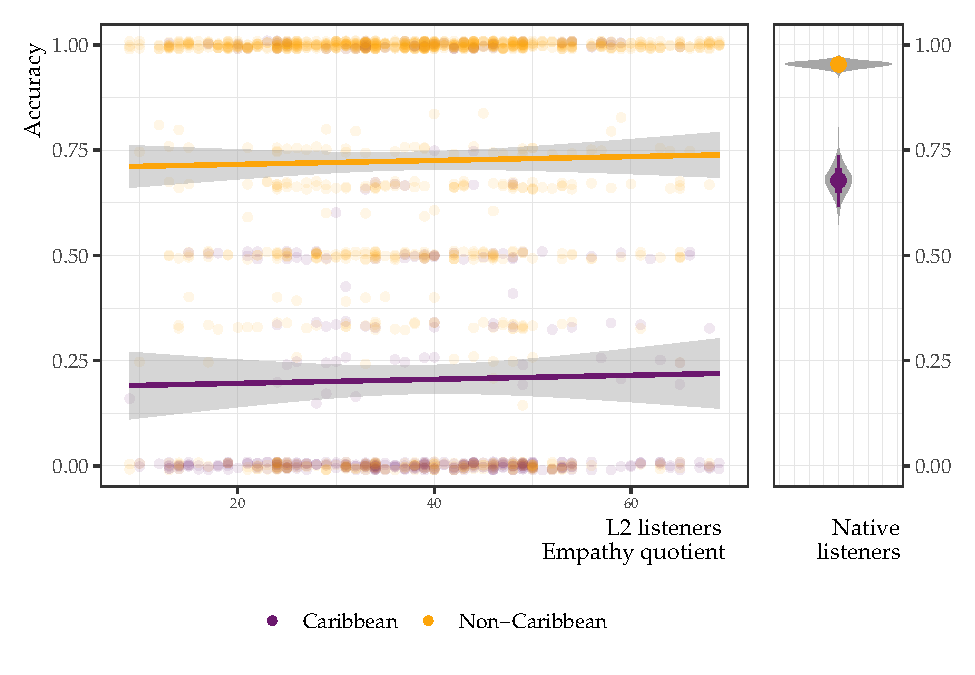
\includegraphics[width=1\linewidth]{../../../../figs/manuscript/learner_native_caribbean_accuracy} \caption{L2 and native listener response accuracy to Caribbean (Cuban, Puerto Rican) and non-Caribbean varieties for yes/no questions. Points represent by-participant means (learners) or posterior means (natives). For learners, the horizontal axis plots empathy quotient scores.}\label{fig:plot-learner-native-caribbean-accuracy}
\end{figure}

\clearpage

The aforementioned information has been incorporated into the discussion section and supplementary materials of the revised manuscript (Table 8 and Figure 10).
We also would like to explicitly acknowledge that while there are still myriad possibilities for further exploratory analyses, we prioritize adhering to our preregistered research protocol.
That being said, we also invite the reviewer (and all future readers) to use our data to run any analyses they deem relevant.
It is precisely for this reason that we make our code and data publicly available.
\Done
\Easy

\clearpage

\hypertarget{reviewer-3}{%
\section{Reviewer \#3}\label{reviewer-3}}

\RC{I think the authors did a great job taking into account our comments and suggestions. The revised version of the manuscript is now much more solid, but I still have some suggestions that I hope can be useful in a new revised version of the manuscript.

The authors now include a lot more details on the listener and speaker dialectal variability and familiarity, but I still feel that this factor is  not well integrated into the manuscript. Here my specific suggestions: 

1) The effect of “speaker variety” on perception accuracy is one of the three research questions of the study, but it is not mentioned in various places in the manuscript where authors summarize their goals. For instance, in p.5, l.5-13 (“we investigated the interplay [...] in L2 Spanish”) the authors include RQ1 and RQ2, but not RQ3. Or in p. 14, l. 815, where the authors state that they aim at extending previous research by considering empathy in L2 sentence processing, but they do not mention the speaker variability/listener familiarity effect.
}

We agree with the reviewer's observations and have modified the introduction as suggested in order to better integrate RQ3 into the revised manuscript.
We include the relevant changes below.

\begin{quote}
Specifically, we investigated the interplay between language proficiency and an individual pragmatic skill (empathy) when learning an L2.
We focused on the role of empathy in the development of L2 prosody by analyzing the perception of intonation in questions and statements in L2 Spanish.
In addition, we considered the role of dialectal variation by exposing listeners to utterances from eight varieties of Spanish.
\end{quote}

\begin{quote}
This project presents a conceptual replication of Brandl, González, and Bustin (2020) in that we employ a similar experimental paradigm using similar stimuli in order to analyze the relationship between proficiency and L2 perception of intonation.
Similar to Brandl et al. (2020), we include speakers from eight different varieties of Spanish in order to consider how dialectal variation influences perceptual development.
We extend this research by taking into account pragmatic skill, specifically empathy, in L2 sentence processing.
Importantly, this research builds on recent studies looking at the role of individual pragmatic skills in language comprehension and extends them to the field of SLA.
\end{quote}

\Done
\Easy

\RC{
2) It still feels strange to have a specific hypothesis about the Cuban variety in the introduction (p. 13, l. 44-45) without any information yet on the pilot or the nature of Cuban intonation. I think it would make more sense to make hypothesis about familiarity. I mean: instead of saying “we hypothesize that L2 learners will have the most difficulty with the Cuban variety”, to say that they will have more difficulty with the variety they are less familiar with, and then in the methods and results we will already learn that this is the Cuban variety.
}

While we agree that the reviewer's suggestion certainly lends itself to a more elegant transition from the research question to the results, collectively we are not comfortable with the idea of hypothesizing after the results are known.
We recognize the temptation to refocus the research question on familiarity, as this seems much more logical \emph{a posteriori}.
Nonetheless, we preregistered our hypothesis about the Cuban variety based on pilot data from monolingual Spanish listeners.
In that sense, we feel that it is sufficiently motivated.
To the reviewer's point, familiarity is clearly relevant and for this reason we expand on it's role on perceptual development in the discussion and the supplementary materials.

\Done
\Easy

\RC{
1) Introduction, p.4, l. 23-25: The authors contrast linguistic information to pragmatic information. Why do the authors think that pragmatics is not part of the linguistic system?
}

The reviewer makes an important point.
We agree that pragmatics is indeed part of the linguistic system and did not intend to suggest otherwise.
In the revised manuscript we have rewritten this sentence to make this more clear.
It now reads as follows:

\begin{quote}
The difficulties associated with intonation can result in comprehension and communication mishaps because the tune is associated with numerous parts of the linguistic system, such as sentence function, e.g., utterance type, syntactic constituency, as well as pragmatic function, e.g., information structure (Casielles-Suárez, 2004; Erteschik-Shir, 2007), speaker belief states (Pierrehumbert \& Hirschberg, 1990), polite discourse (Astruc, Vanrell, \& Prieto, 2016), bias, or presupposition (Henriksen, Armstrong, \& García-Amaya, 2016).
\end{quote}

\Done
\Easy

\RC{
2) Figure 5, left panel: should the title of the graph be “b-accuracy” instead of “b-response”?
}

We have included this change in the revised manuscript.

\Done
\Easy

\RC{
3) p. 31, last line: change “que” for “qué” in “Qué bebe María?”. While the same pronoun is used, one is tonic and the other one not, so the nature of the “que” could have guided participants’ choices.
}

This oversight was also pointed out by reviewer 2.
We have included this change in the revised manuscript.
The sentence in question now reads as follows:

\begin{quote}
That is to say, in specific contexts these same words can appear in statements as well, in some cases with a pitch accent (i.e., \emph{Qué beba María}) and in others without (i.e., \emph{Que bebe María}).
\end{quote}

\Done
\Easy

\newpage

\hypertarget{references}{%
\section{References}\label{references}}

\hypertarget{refs}{}
\begin{CSLReferences}{1}{0}
\leavevmode\vadjust pre{\hypertarget{ref-armstrong2010puerto}{}}%
Armstrong, M. E. (2010). Puerto {R}ican {S}panish intonation. In P. Prieto \& P. Roseano (Eds.), \emph{Transcription of intonation of the {S}panish language} (pp. 155--189). Münich: Lincom Europa.

\leavevmode\vadjust pre{\hypertarget{ref-Armstrong2017}{}}%
Armstrong, M. E. (2017). Accounting for intonational form and function in {P}uerto {R}ican {S}panish polar questions. \emph{Probus}, \emph{29}(1), 1--40. \url{https://doi.org/10.1515/probus-2014-0016}

\leavevmode\vadjust pre{\hypertarget{ref-astruc2016cost}{}}%
Astruc, L., Vanrell, M., \& Prieto, P. (2016). Cost of the action and social distance affect the selection of question intonation in {C}atalan. In M. E. Armstrong, N. Henriksen, \& M. Vanrell (Eds.), \emph{Intonational grammar in {I}bero-{R}omance: {A}pproaches across linguistic subfields} (pp. 93--113). John Benjamins Publishing Company. \url{https://doi.org/10.1075/ihll.6}

\leavevmode\vadjust pre{\hypertarget{ref-bustin_2020}{}}%
Brandl, A., González, C., \& Bustin, A. (2020). The development of intonation in {L}2 {S}panish: {A} perceptual study. In A. Morales-Front, M. J. Ferreira, R. P. Leow, \& C. Sanz (Eds.), \emph{Hispanic linguistics: Current issues and new directions} (pp. 12--31). John Benjamins Publishing Company. \url{https://doi.org/10.1075/ihll.26}

\leavevmode\vadjust pre{\hypertarget{ref-casielles2004syntax}{}}%
Casielles-Suárez, E. (2004). \emph{The syntax-information structure interface: {E}vidence from {S}panish and {E}nglish}. Routledge.

\leavevmode\vadjust pre{\hypertarget{ref-erteschik2007information}{}}%
Erteschik-Shir, N. (2007). \emph{Information structure: {T}he syntax-discourse interface} (Vol. 3). OUP Oxford.

\leavevmode\vadjust pre{\hypertarget{ref-gabriel2010argentine}{}}%
Gabriel, C., Feldhausen, I., Pešková, A., Colantoni, L., Lee, S., Arana, V., \& Labastía, L. (2010). {A}rgentinian {S}panish intonation. In P. Prieto \& P. Roseano (Eds.), \emph{Transcription of intonation of the {S}panish language} (pp. 285--317). Münich: Lincom Europa.

\leavevmode\vadjust pre{\hypertarget{ref-henriksen2016intonational}{}}%
Henriksen, N., Armstrong, M. E., \& García-Amaya, L. J. (2016). The intonational meaning of polar questions in {M}anchego {S}panish spontaneous speech. In M. E. Armstrong, N. Henriksen, \& M. del M. Vanrell (Eds.), \emph{Intonational grammar in {I}bero-{R}omance: {A}pproaches across linguistic subfields} (pp. 181--205). John Benjamins Publishing Company. \url{https://doi.org/10.1075/ihll.6}

\leavevmode\vadjust pre{\hypertarget{ref-hualde2015intonational}{}}%
Hualde, J. I., \& Prieto, P. (2015). Intonational variation in {S}panish: {E}uropean and {A}merican varieties. In S. Frota \& P. Prieto (Eds.), \emph{Intonation in {R}omance} (pp. 350--391). Oxford University Press.

\leavevmode\vadjust pre{\hypertarget{ref-ladd2008intonational}{}}%
Ladd, D. R. (2008). \emph{Intonational phonology}. Cambridge University Press.

\leavevmode\vadjust pre{\hypertarget{ref-marasco2020you}{}}%
Marasco, O. M. (2020). \emph{{``Are you asking me or telling me?''} {P}erception and production of {Y/N} questions and statements in {L}2 {S}panish} (PhD thesis). University of Toronto.

\leavevmode\vadjust pre{\hypertarget{ref-mennen2015beyond}{}}%
Mennen, I. (2015). Beyond segments: {T}owards a {L}2 intonation learning theory. In \emph{Prosody and language in contact} (pp. 171--188). Springer. \url{https://doi.org/10.1007/978-3-662-45168-7_9}

\leavevmode\vadjust pre{\hypertarget{ref-ortiz2003acentos}{}}%
Ortiz-Lira, H. (2003). Los acentos tonales en un corpus de {E}spañol de {Santiago de Chile}: Su distribución y realización. \emph{La Tonía: Dimensiones Fonéticas y Fonológicas}, 303--316.

\leavevmode\vadjust pre{\hypertarget{ref-lira2000prosodia}{}}%
Ortiz-Lira, H., \& Cid-Uribe, M. E. (2000). La prosodia de las preguntas indagativas y no-indagativas del {E}spañol culto de {S}antiago de {C}hile. \emph{LEA: Lingüística {E}spañola {A}ctual}, \emph{22}(1), 23--49.

\leavevmode\vadjust pre{\hypertarget{ref-pierrehumbert1980phonology}{}}%
Pierrehumbert, J. (1980). \emph{The phonology and phonetics of {E}nglish intonation} (PhD thesis). Massachusetts Institute of Technology.

\leavevmode\vadjust pre{\hypertarget{ref-pierrehumbert1990meaning}{}}%
Pierrehumbert, J., \& Hirschberg, J. (1990). The meaning of intonational contours in the interpretation of discourse. In P. R. Cohen, J. L. Morgan, \& M. E. Pollack (Eds.), \emph{Intentions in communication} (pp. 271--312). {MIT} press.

\leavevmode\vadjust pre{\hypertarget{ref-alvarado2022prosodic}{}}%
Sánchez Alvarado, C., \& Armstrong, M. (2022). Prosodic marking of object focus in {L}2 {S}panish. \emph{Studies in Hispanic and Lusophone Linguistics}, \emph{15}(1), 211--250. \url{https://doi.org/10.1515/shll-2022-2060}

\leavevmode\vadjust pre{\hypertarget{ref-sanchez2022acquisition}{}}%
Sánchez-Alvarado, C. (2022). The acquisition of {L}2 {S}panish intonation: {A}n analysis based on features. \emph{Journal of Second Language Pronunciation}, \emph{8}(1), 40--67. \url{https://doi.org/10.1075/jslp.20041.san}

\leavevmode\vadjust pre{\hypertarget{ref-willis2010dominican}{}}%
Willis, E. W. (2010). {D}ominican {S}panish intonation. In P. Prieto \& P. Roseano (Eds.), \emph{Transcription of intonation of the {S}panish language} (pp. 123--153). Münich: Lincom Europa.

\end{CSLReferences}


\end{document}\grid
